\section{EMIM-TFSI with NaTFSI or LiTFSI solutions}

This section describes structural results obtained from classical MD for series of electrolytes based on LiTFSI or NaTFSI dissolved in EMIM-TFSI ionic liquids. This is a~part of a~study published in paper~\cite{li-na} aimed at investigating the correlations in the motions of ions in salt solutions in ILs. Such correlations can affect the conductivity of the electrolyte. They were broadly studied experimentally, for example, for lithium-based ILs~\cite{li-na-exp-1,li-na-exp-2,li-na-exp-3}, for lithium salts dissolved in glymes~\cite{li-na-exp-4,li-na-exp-5} or for electrolytes with carbonates as solvents~\cite{li-na-exp-6}. The research on this topic also involved theoretical studies with the use of MD methods~\cite{li-na-continuation,li-na-md-1,li-na-md-2,li-na-md-3}.

\subsection{System details}
\label{subsection:li-na-system-details}

Five systems Me$_x$EMIM$_{1-x}$TFSI with Me = Li or Na and x equal 0.0, 0.06, 0.12, 0.2 and 0.3 were investigated. Their compositions are listed in Table~\ref{tab:li-na-compositions}.

\begin{table}[ht]
    \centering
    \caption{Compositions of Me$_{x}$EMIM$_{1-x}$TFSI systems}
    \label{tab:li-na-compositions}
    \begin{tabular}{cccc}
      \toprule
      x & Me$^{+}$ & EMIM$^{+}$ & FSI$^{-}$ \\
      \midrule
      0 & 0 & 142 & 142 \\
      0.06 & 10 & 148 & 158 \\
      0.12 & 20 & 141 & 161 \\
      0.2 & 32 & 128 & 160 \\
      0.3 & 51 & 119 & 170 \\
      \bottomrule
    \end{tabular}    
\end{table}

For classical MD pressure $p = 1$~atm and temperature $T = 333$~K were used. After 100~ns of equilibration trajectories for all systems were recorded for 1000~ns in simulations using DP-FF and NP-FF with a~time step of 1.0~fs.

\subsection{Results}

The RDFs for the Me-O distances are shown in Figure~\ref{fig:li-na-fig-1}. The positions of the peaks do not change significantly with salt concentration and are located at 2.0~{\AA} and 2.1~{\AA} for lithium in DP-FF and NP-FF respectively, while for sodium maxima appear at at 2.5~{\AA} and 2.6~{\AA}. The longer distances for sodium as well as the fact that its maxima are lower and wider than those of lithium, are caused by the larger radius of the Na$^{+}$ ion. 

Coordination numbers are determined from the integrated RDFs at the distance of 3~{\AA} for lithium and are equal 3.96 in DP-FF and 4.76 in NP-FF and for the distance of 3.5~{\AA} for sodium and are equal 5.34 and 5.66 respectively. The differences are related to the stronger Me-anion interactions in the polarizable simulations --- maxima of the RDFs are shifted towards lower distances, so the solvation shell is tighter.

Figure~\ref{fig:li-na-fig-2} presents the abundance of the number of oxygen atoms or anions that coordinate the metal cation, respectively. Me$^{+}$ cation is treated as coordinated to the oxygen atom if its distance at a given moment is lower than threshold value: 3.0~{\AA} for lithium and 3.5~{\AA} for sodium. In DP-FF, most lithium ions are coordinated by 4~oxygen atoms from 2~anions, which suggests that coordination is bidentate. For sodium cations, the most probable number of coordinating atoms are 5~and~6 from~3 anions, thus in sodium electrolytes most of metal cations are coordinated either as bidentate by two anions and as monodentate by the 3rd anion, or in bidentate manner by 3~anions. In NP-FF coordination numbers are shifted towards higher values - 5~for lithium and 6~for sodium. Both types of cation are in this case predominantly coordinated by 4~anions. Therefore, it seems that NP-FF favorizes monodentate binding in complexes. The DP-FF results agree with the structures obtained experimentally~\cite{li-na-exp-1}.

\begin{figure}[H]
    \centering
    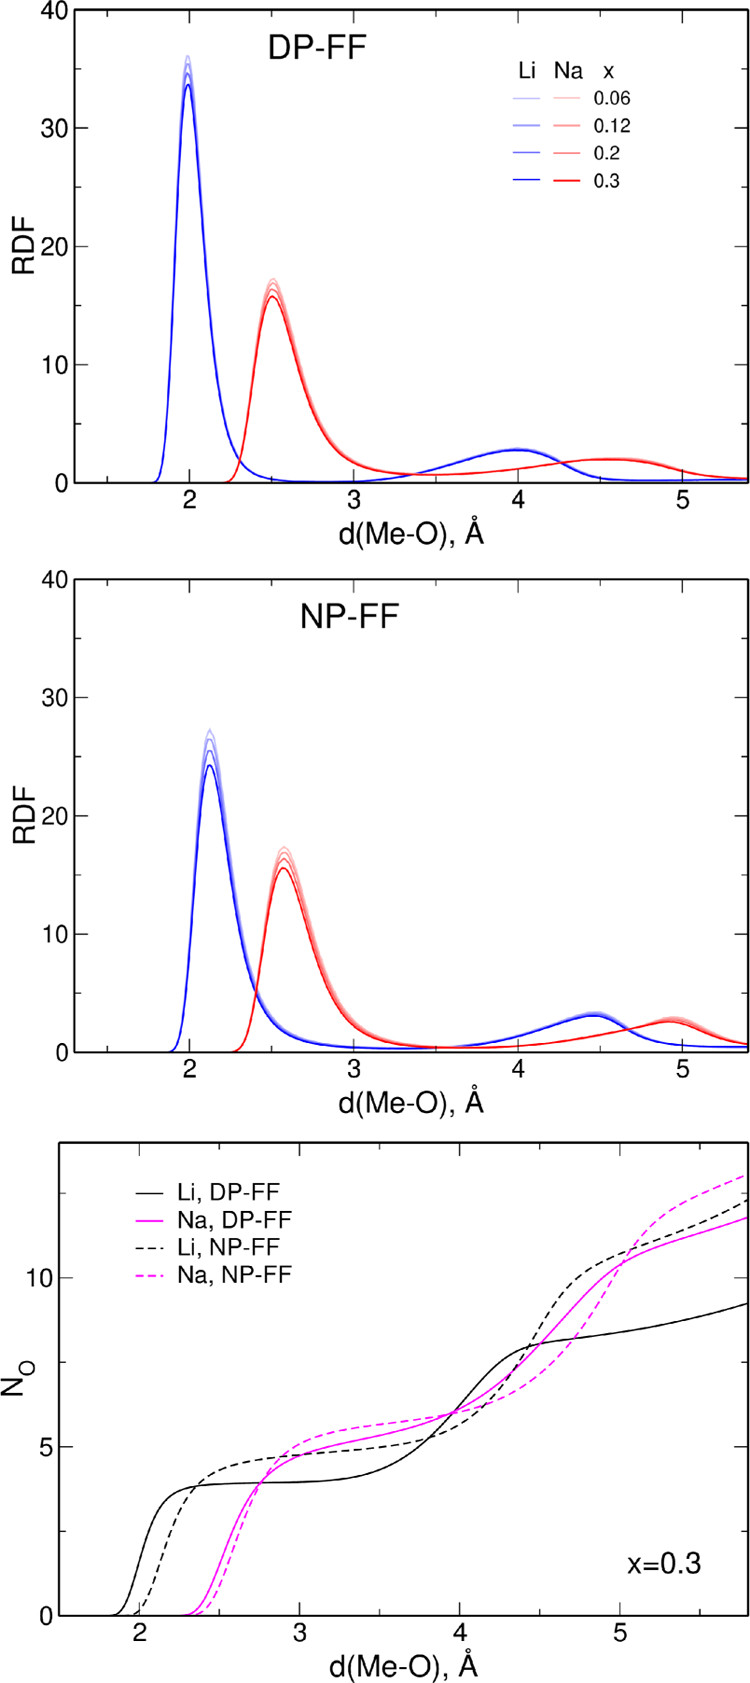
\includegraphics[width=0.45\textwidth]{img/3-structural-data-from-md-simulations/2-li-na/fig1.png}
    \caption{Radial distribution functions for Me-O distances in the polarizable (top) and nonpolarizable (middle) FF and the running coordination numbers for Me-O (bottom) for the system with $x = 0.3$}
    \label{fig:li-na-fig-1}
\end{figure}

Residence time autocorrelation functions are plotted in Figure~\ref{fig:li-na-fig-4}. The decay of this function is slower for lithium ions, which is caused by stronger interaction between the Li$^{+}$ cation and the TFSI$^{-}$ anion due to the smaller size of the former. Increasing salt concentration further slows the decay (except for sodium in DP-FF). For each of the data series, a~stretched exponential function $e^{-\left(\frac{t}{\tau_O}\right)^{\alpha}}$ was fitted, the residence times obtained $\tau$ for individual oxygen atoms and for whole anions are presented at the bottom of Figure~\ref{fig:li-na-fig-4}. Residence times for anions are 3-10 times larger than values for oxygen atoms, and this is due to the fact that exchange of the anion requires breaking all of the interactions from its oxygen atoms to the cation. Values for lithium are 4-8 times higher than those for sodium and are more dependent on salt concentration. These results indicate that anion exchange in the sodium solvation shell is faster than for lithium.

\begin{figure}[H]
    \centering
    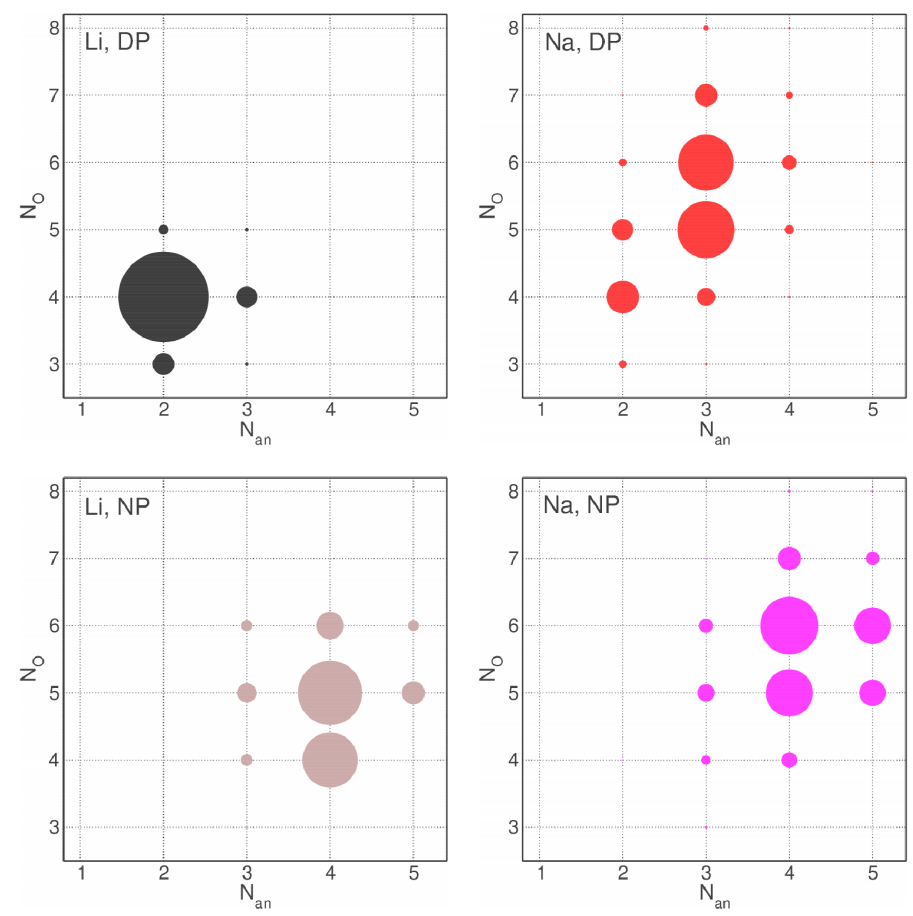
\includegraphics[width=0.65\textwidth]{img/3-structural-data-from-md-simulations/2-li-na/fig2.png}
    \caption{Abundance of different combinations of the number of anions $N_{\text{an}}$ and the number of oxygen atoms $N_{\text{O}}$ coordinating Me$^{+}$ ions in NP-FF and DP-FF; areas of the circles are proportional to the abundance}
    \label{fig:li-na-fig-2}
\end{figure}

\begin{figure}[ht]
    \centering
    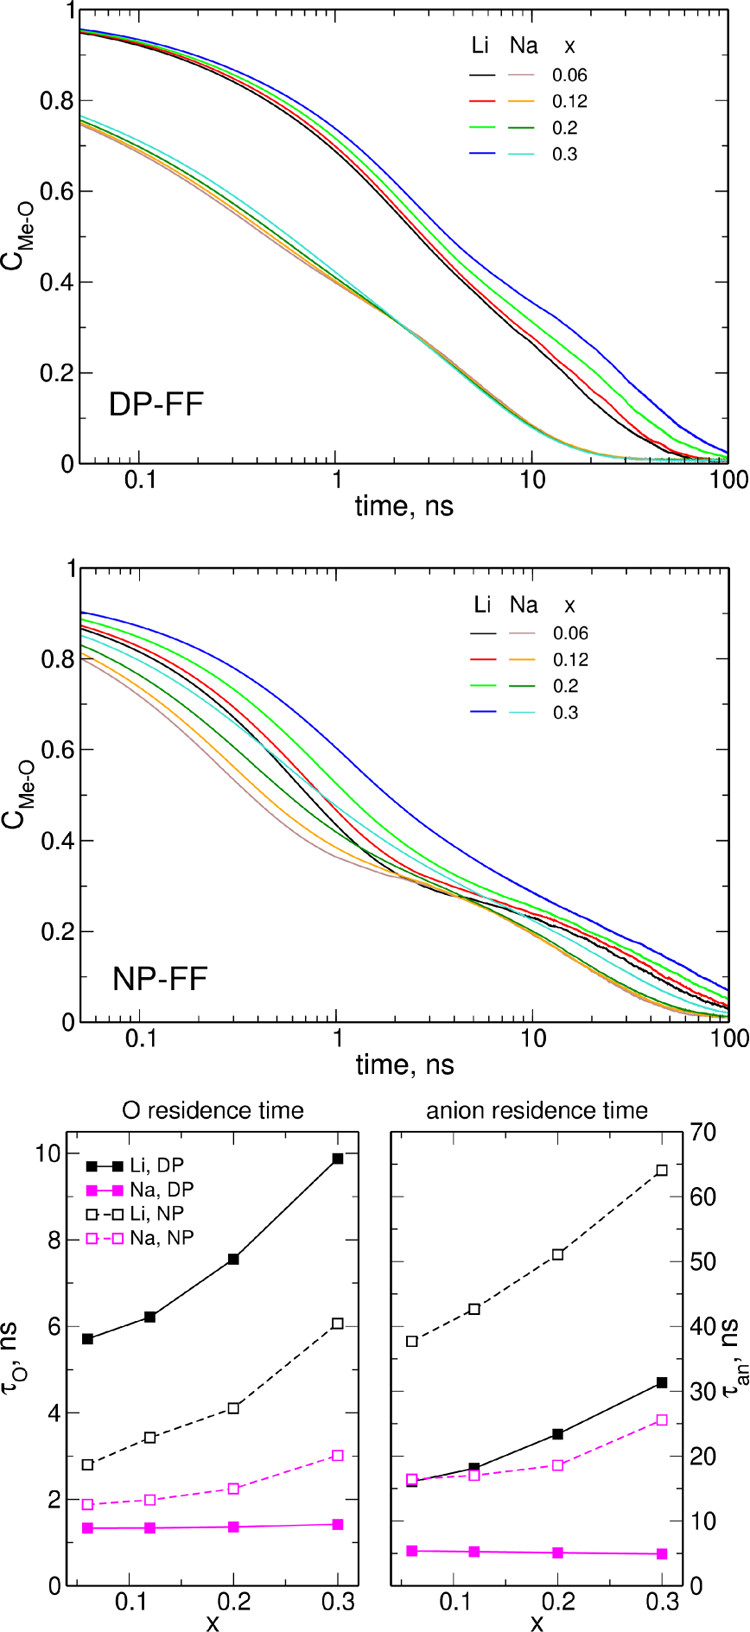
\includegraphics[width=0.5\textwidth]{img/3-structural-data-from-md-simulations/2-li-na/fig4.png}
    \caption{Residence time autorcorrelation functions for Me-O for DP-FF (top), NP-FF (middle) and $\tau$ parameters for O~atoms and TFSI~anions (bottom)}
    \label{fig:li-na-fig-4}
\end{figure}

The structural data presented in this section show remarkable differences in the structure and dynamics of the solvation shell of Li$^{+}$ and Na$^{+}$ in EMIM-TFSI as well as the dependence of the results on the FF used in the simulations. Nevertheless, further analysis of ion transport and conductivity in~\cite{li-na} resulted in the conclusion that regardless of the cation or the type of FF, correlations between ion motions lead to negative Me$^{+}$ transference numbers in salt solutions in ILs.

\cleardoublepage